\section{Shape-Diverse DSLs}
\label{sec:shapes}

The cornerstone artifact defining a DSL in any LV is its abstract syntax.
The way abstract syntax is expressed differs drastically from one LV to another: GEMOC~\cite{bousse2016execution} and Xtext~\cite{bettini2016implementing} use Ecore metamodels~\cite{steinberg2008emf}; MPS~\cite{voelter2014generic} uses \emph{concepts}; Rascal~\cite{klint2010easy} uses Algebraic Data Types (ADT); \etc.
Language embedding techniques, on the other hand, use the constructs of an host language to materialize the constructs of a DSL in the host language itself (\eg~a set of Java classes).
Concrete models are then built as instances of the corresponding abstract syntax formalism:~Ecore models, ADT values, Java ASTs, \etc.
The tools defined within a particular LV (an interpreter in Rascal, an editor in EMF) manipulate models in the corresponding formalism (respectively, ADT values and Ecore models).
These formalisms radically differ in many ways~\cite{klint2016model}:~object-oriented vs. functional, graphs vs. trees, mutable ASG vs. immutable ASTs, cross-references vs. symbolic names, \etc.
As LVs are developed by independent groups of people and rely on different underlying theories, it is neither possible nor desirable to establish a common foundation upon which all LVs would agree.

\begin{figure}[bt]
	\centering
	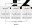
\includegraphics[width=.7\columnwidth]{figures/shape-diverse-lang-3}
	\caption{Languages are implemented as shapes in LVs and models are projected as incarnations conforming to the shapes.}
	\label{fig:concepts}
\end{figure}

\Cref{fig:concepts} gives an overview of the concept of shape-diverse language and the terminology we use throughout the paper.
A shape-diverse language $\mathcal{L}$ (\eg~the FSM language of \Cref{fig:motivating-fsm}) is a language that is implemented in multiple LV through multiple shapes $\mathcal{S}_i$.
%A ``conceptual'' language $\mathcal{L}$ is materialized as a \emph{shape} $\mathcal{S}$ in a LV.
Each $\mathcal{S}_i$ can therefore be seen as the implementation of $\mathcal{L}$ in LV\textsubscript{i}.
As mentioned earlier, Ecore metamodels, ADT definitions, and Java APIs, along with their associated tooling, are examples of shapes.
Similarly, a ``conceptual'' model $m$ that uses the constructs of $\mathcal{L}$ (\eg~the simple {\footnotesize \texttt{Button}} machine) is projected as an incarnation $\mathcal{I}_i$ conforming to the shape $\mathcal{S}_i$ in a LV\textsubscript{i}: an Ecore model, an ADT value, or a Java AST.
%\td{Not very proud of the ``conceptual''. Is ``abstract'' better? Any idea?}
%\fc{Language Specification and Abstract Model?} 
%As each shape manipulate models in its own formalism, all incarnations $I$ of the same model $m$ must remain synchronized.

%An obvious way to bridge different LVs would be to define bidirectional transformations between the abstract syntax formalisms of every pair $\langle LV, LV' \rangle$.
%Doing so however would close the world around the chosen set of LVs.
%As every LV holds particular extra information on its incarnations, such as layout in an editor, runtime data for running models, or context information around API calls, the synchronization must be incremental.

As each shape manipulates models in its own formalism, all incarnations $\mathcal{I}_i$ of the same model $m$ must remain synchronized.
This synchronization mechanism must ensure two important properties.
First, it must not close the world around a chosen set of LVs:~it should be possible to easily connect new LVs and shapes to meet new requirements from users and designers.
This rules out any synchronization approach that would require to be defined for every pair $\langle LV, LV' \rangle$, such as bidirectional transformations. \td{Debatable}
Second, it must account for any extra shape-specific information the various LVs have to maintain to function properly.
Examples of such extra information include layout information in a textual or graphical editor, or runtime state in a simulation environment.
Every LV should be able to update its own incarnation while maintaining this extra information.
